\setAuthor{Kaarel Kivisalu}
\setRound{lahtine}
\setYear{2021}
\setNumber{G 10}
\setDifficulty{10}
\setTopic{TODO}

\prob{Kolmnurk}
Traadist on tehtud võrdkülgne kolmnurk, mille sisse on pandud lõputult palju samast traadist tehtud võrdkülgseid kolmnurki (vt joonist). Traadi takistus pikkusühiku kohta on selline, et kolmnurga $ABC$ ühe külje takistus on $R$. Leidke kolmnurga $ABC$ tippude $A$ ja $B$ vaheline takistus.

\begin{figure}[h]
  \centering
  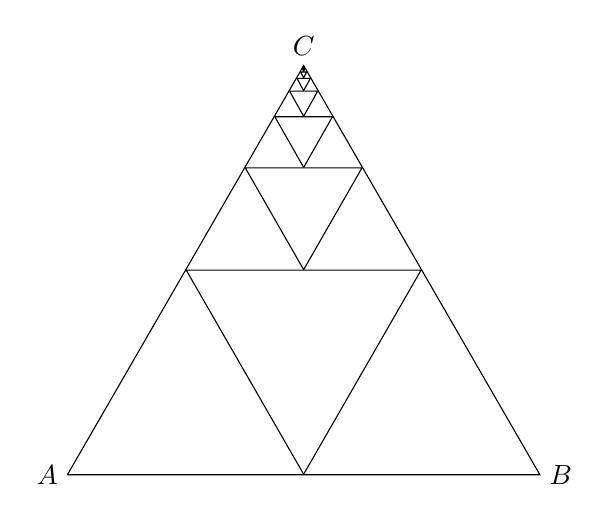
\begin{tikzpicture}[scale=3]
    \draw (0,0) node[left] {$A$} -- (2,0) node[right] {$B$}-- (1, 1.732) node[above] {$C$} -- (0,0);
    \foreach \x in {0,...,7}
    {
      \draw[line cap = round] (1, 1.734-1.732/2^\x) -- (1.003-0.5/2^\x,1.732-0.866/2^\x) -- (0.997+0.5/2^\x,1.732-0.866/2^\x) -- (1, 1.734-1.732/2^\x);
    }
  \end{tikzpicture}
\end{figure}


\hint

\solu
Märkame, et $A'B'C$ on sarnane kolmnurgaga $ABC$, kuid 2 korda väiksem. Seega saame asendada kolmnurga $A'B'C$ takistiga mille takistus on pool otsitavast takistusest: $\frac{R_{AB}}{2}$. Saame järgneva ekvivalentskeemi:

\begin{figure}[h]
\centering

  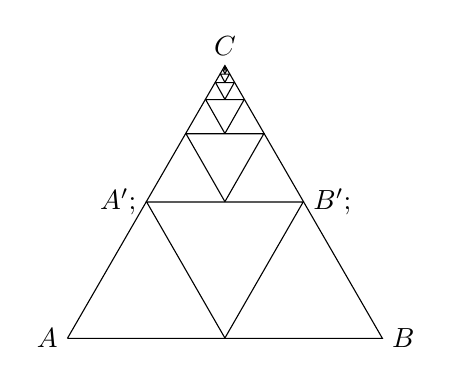
\begin{tikzpicture}[scale=2]
    \draw (0,0) node[left] {$A$} -- (2,0) node[right] {$B$} -- (1.5,0.866) node[right] {$B';$} -- (1, 1.732) node[above] {$C$} -- (0.5,0.866) node[left] {$A';$} -- (0,0);

    \foreach \x in {0,...,7}
    {
      \draw[line cap = round] (1, 1.734-1.732/2^\x) -- (1.003-0.5/2^\x,1.732-0.866/2^\x) -- (0.997+0.5/2^\x,1.732-0.866/2^\x) -- (1, 1.734-1.732/2^\x);
    }
  \end{tikzpicture}
  \begin{circuitikz}[scale=3]
    \draw (0,0) node[left] {$A$} to[R=$R/2$] (1,0) to[R=$R/2$] (2,0) node[right] {$B$} to[R=$R/2$] (1.5,0.866) node[right] {$B'$} to[R=$R_{AB}/2$] (0.5,0.866) node[left] {$A'$} to[R=$R/2$] (0,0);

    \draw (0.5,0.866) to[R=$R/2$] (1,0) to[R=$R/2$] (1.5,0.866);
  \end{circuitikz}
\end{figure}

Skeem on kesktelje suhtes sümmeetriline, seega on kogutakistus
\begin{align}
  R_{AB}&=2\left[\frac{1}{\frac{R}{2}}+\left(\frac{R}{2} + \frac{\frac{R}{2}\frac{R_{AB}}{4}}{\frac{R}{2}+\frac{R_{AB}}{4}}\right)^{-1}\right]^{-1}\\
        &= 2 \left[ \frac{1}{\frac{R}{2}} + \left( \frac{\frac{R}{2} \frac{R}{2} + \frac{R}{2} \frac{R_{AB}}{4} + \frac{R}{2}\frac{R_{AB}}{4}}{\frac{R}{2}+\frac{R_{AB}}{4}} \right)^{-1} \right]^{-1}\\
        &= 2 \left[ \frac{1}{\frac{R}{2}} +  \frac{\frac{R}{2}+\frac{R_{AB}}{4}}{\frac{R}{2}\left(\frac{R}{2}+ \frac{R_{AB}}{2}\right)}  \right]^{-1}\\
        &= 2 \left[ \frac{R+\frac{3}{4}R_{AB}}{\frac{R}{2}\left(\frac{R}{2}+ \frac{R_{AB}}{2}\right)}  \right]^{-1}\\
        &= \frac{2R(R + R_{AB})}{4R+3R_{AB}}.
\end{align}
Seega
\begin{align}
&4R R_{AB} +3 R_{AB}^2=2R^2+2R R_{AB}\\
  \implies& 3R_{AB}^2 +2 R R_{AB} - 2R^2=0 \\
  \implies& R_{AB}=\frac{-2R \pm \sqrt{4R^2+24R^2}}{6}=\frac{\pm\sqrt{7}-1}{3}R.
\end{align}
Kuna peab kehtima, et $R_{AB} \geq 0$, siis
\begin{equation}
R_{AB}= \frac{\sqrt{7}-1}{3} R.
\end{equation}
\probend